\documentclass[12pt,a4paper]{article}

\usepackage[utf8]{inputenc}
\usepackage[T1]{fontenc}
\usepackage[margin=2.5cm]{geometry}
\usepackage{amsmath, amssymb}
\usepackage{xcolor}
\usepackage{tikz}
\usetikzlibrary{shapes.geometric, arrows.meta, positioning}
\usepackage{booktabs}
\usepackage{listings}
\usepackage{hyperref}
\usepackage{enumitem}

\hypersetup{colorlinks=true, linkcolor=blue!70!black}

\lstset{
  basicstyle=\ttfamily\small,
  keywordstyle=\color{blue!80!black}\bfseries,
  commentstyle=\color{green!50!black}\itshape,
  stringstyle=\color{red!70!black},
  backgroundcolor=\color{gray!8},
  frame=single, framerule=0.4pt,
  breaklines=true,
  numbers=left, numberstyle=\tiny\color{gray},
  numbersep=6pt, language=Python
}

\definecolor{structcolor}{HTML}{2196F3}
\definecolor{soilcolor}{HTML}{8D6E63}
\definecolor{loadcolor}{HTML}{FF5722}
\definecolor{envcolor}{HTML}{00BCD4}
\definecolor{fusioncolor}{HTML}{9C27B0}

\title{\textbf{Meeting 2 — Specialized-Slot Yield Transformer}\\[0.3em]
\large Architecture \& Code Walkthrough}
\author{PFE Research Notes}
\date{March 2026}

\begin{document}
\maketitle
\tableofcontents
\newpage

% ===========================================================
\section{Architecture Diagram}
% ===========================================================

\begin{figure}[h]
\centering
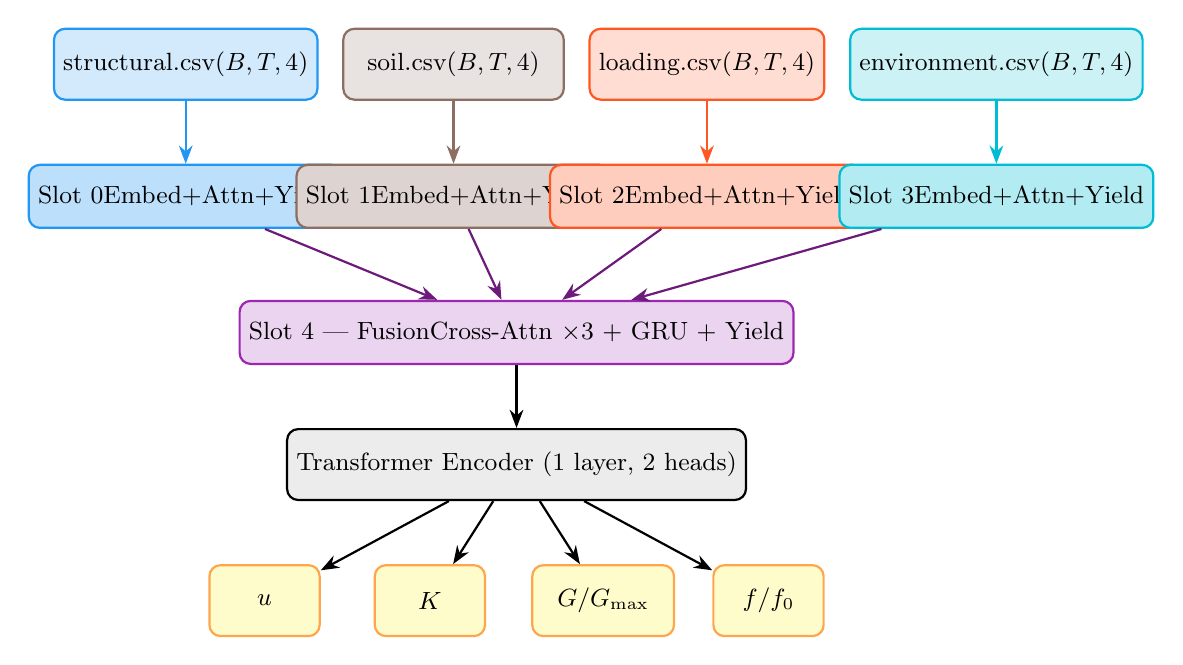
\begin{tikzpicture}[
  node distance=0.6cm and 0.9cm,
  box/.style={rectangle, rounded corners=4pt, draw, thick,
              minimum width=2.8cm, minimum height=0.9cm,
              text centered, font=\small},
  arrow/.style={->, thick, >=Stealth},
  slot/.style={box, minimum width=2.4cm, minimum height=0.8cm},
]
\node[box, fill=structcolor!20, draw=structcolor] (S) {structural.csv\\$(B,T,4)$};
\node[box, fill=soilcolor!20,   draw=soilcolor,   right=0.3cm of S]  (So){soil.csv\\$(B,T,4)$};
\node[box, fill=loadcolor!20,   draw=loadcolor,   right=0.3cm of So] (L) {loading.csv\\$(B,T,4)$};
\node[box, fill=envcolor!20,    draw=envcolor,    right=0.3cm of L]  (E) {environment.csv\\$(B,T,4)$};

\node[slot, fill=structcolor!30, draw=structcolor, below=0.8cm of S]  (SS) {Slot 0\\Embed+Attn+Yield};
\node[slot, fill=soilcolor!30,   draw=soilcolor,   below=0.8cm of So] (SoS){Slot 1\\Embed+Attn+Yield};
\node[slot, fill=loadcolor!30,   draw=loadcolor,   below=0.8cm of L]  (LS) {Slot 2\\Embed+Attn+Yield};
\node[slot, fill=envcolor!30,    draw=envcolor,    below=0.8cm of E]  (ES) {Slot 3\\Embed+Attn+Yield};

\draw[arrow, structcolor] (S)--(SS);
\draw[arrow, soilcolor]   (So)--(SoS);
\draw[arrow, loadcolor]   (L)--(LS);
\draw[arrow, envcolor]    (E)--(ES);

\node[slot, fill=fusioncolor!20, draw=fusioncolor, minimum width=4.5cm,
      below=0.9cm of SoS, xshift=0.8cm] (FS) {Slot 4 — Fusion\\Cross-Attn $\times3$ + GRU + Yield};

\draw[arrow, fusioncolor!70!black] (SS)--(FS);
\draw[arrow, fusioncolor!70!black] (SoS)--(FS);
\draw[arrow, fusioncolor!70!black] (LS)--(FS);
\draw[arrow, fusioncolor!70!black] (ES)--(FS);

\node[box, fill=gray!15, below=0.8cm of FS, minimum width=5cm] (TE)
     {Transformer Encoder (1 layer, 2 heads)};
\draw[arrow] (FS)--(TE);

\node[box, fill=yellow!20, draw=orange!70, below=0.8cm of TE, xshift=-3.2cm, minimum width=1.4cm] (Ou){$u$};
\node[box, fill=yellow!20, draw=orange!70, below=0.8cm of TE, xshift=-1.1cm, minimum width=1.4cm] (OK){$K$};
\node[box, fill=yellow!20, draw=orange!70, below=0.8cm of TE, xshift=+1.1cm, minimum width=1.8cm] (OG){$G/G_\text{max}$};
\node[box, fill=yellow!20, draw=orange!70, below=0.8cm of TE, xshift=+3.2cm, minimum width=1.4cm] (Of){$f/f_0$};

\draw[arrow](TE)--(Ou); \draw[arrow](TE)--(OK);
\draw[arrow](TE)--(OG); \draw[arrow](TE)--(Of);
\end{tikzpicture}
\caption{Full architecture: 4 specialized slots $\to$ fusion slot $\to$ encoder $\to$ 4 output heads.}
\label{fig:arch}
\end{figure}

% ===========================================================
\section{Yield-Surface Activation (Core Novelty)}
% ===========================================================

Every slot uses a custom activation inspired by the Ramberg--Osgood yield model:
\begin{equation}
  f(x) = \frac{x}{\left(1+\left|\frac{x}{\sigma_y}\right|^p\right)^{1/p}}
  \label{eq:yield}
\end{equation}

\begin{itemize}[nosep]
  \item $\sigma_y$ (yield point) and $p$ (sharpness) are \textbf{learned} via backpropagation.
  \item $|x|\ll\sigma_y$: output $\approx x$ (linear / elastic).
  \item $|x|\gg\sigma_y$: output $\to\pm\sigma_y$ (saturated / plastic).
\end{itemize}

\begin{lstlisting}[caption={YieldActivation — the physics-inspired activation.}]
class YieldActivation(nn.Module):
    def __init__(self, dim):
        super().__init__()
        # Raw parameters — transformed to positive via softplus
        self.sigma_y_raw = nn.Parameter(torch.randn(dim) * 0.1)
        self.p_raw       = nn.Parameter(torch.zeros(1))

    def forward(self, x):
        sigma_y = F.softplus(self.sigma_y_raw) + 0.01   # ensure > 0
        p       = 1.5 + F.softplus(self.p_raw)           # ensure > 1.5
        ratio   = (x / sigma_y).abs().clamp(max=15.0)
        return x / (1.0 + ratio.pow(p)).pow(1.0 / p)
\end{lstlisting}

\texttt{softplus} maps any real number to a positive number, guaranteeing $\sigma_y>0$ and $p>1.5$.
Each of the 5 slots learns its own $\sigma_y$ and $p$, so the structural slot's yield threshold differs from the soil slot's — matching real physics.

% ===========================================================
\section{Specialized Slot (one per domain)}
% ===========================================================

Each slot sees \textbf{only its own CSV data} and performs three steps:

\begin{enumerate}[nosep]
  \item \textbf{Embed} the 4 raw features into a 32-dim vector.
  \item \textbf{Self-attention} across the 30 time steps to find temporal patterns.
  \item \textbf{Yield activation} to cap signals at the domain's learned threshold.
\end{enumerate}

\begin{lstlisting}[caption={SpecializedSlot — one domain expert.}]
class SpecializedSlot(nn.Module):
    def __init__(self, n_features, name="slot"):
        super().__init__()
        self.name = name

        # Step 1: domain embedding  (4 raw features -> 32-dim)
        self.embed = nn.Sequential(
            nn.Linear(n_features, D_MODEL),  # 4 -> 32
            nn.ReLU(),
            nn.Linear(D_MODEL, D_MODEL),     # 32 -> 32
        )

        # Step 2: self-attention over time (2 heads)
        self.self_attn = nn.MultiheadAttention(
            D_MODEL, num_heads=2, batch_first=True, dropout=0.1)
        self.norm = nn.LayerNorm(D_MODEL)

        # Step 3: yield activation for this domain
        self.yield_act = YieldActivation(D_MODEL)

    def forward(self, x):           # x: (B, T, 4)
        h = self.embed(x)           # (B, T, 32) - embed
        h_n = self.norm(h)
        h_sa, _ = self.self_attn(h_n, h_n, h_n)  # self-attention
        h = h + h_sa                # residual connection
        h = self.yield_act(h)       # yield filter
        return h                    # (B, T, 32)
\end{lstlisting}

Output shape: $(B, T, 32)$ — a 32-number representation at each of the 30 time steps per scenario.

% ===========================================================
\section{Fusion Slot (combines all 4 domains)}
% ===========================================================

The fusion slot takes \textbf{all four slot outputs} and merges them via cross-attention:

\begin{enumerate}[nosep]
  \item A learnable \textbf{query} asks ``what matters now?''
  \item \textbf{Cross-attention} computes weights $\alpha_i$ over the 4 domains.
  \item A \textbf{GRU} blends the result with the previous state.
  \item Steps 1--3 repeat 3 times (iterative refinement).
  \item A final \textbf{yield activation} filters the fused signal.
\end{enumerate}

\begin{lstlisting}[caption={FusionSlot — cross-attention over the 4 specialist slots.}]
class FusionSlot(nn.Module):
    def __init__(self):
        super().__init__()
        self.cross_attn = nn.MultiheadAttention(
            D_MODEL, num_heads=2, batch_first=True, dropout=0.1)
        self.norm_q  = nn.LayerNorm(D_MODEL)
        self.norm_kv = nn.LayerNorm(D_MODEL)

        # Learnable initial query
        self.fusion_query = nn.Parameter(
            torch.randn(1, 1, D_MODEL) * 0.02)

        # GRU for iterative refinement
        self.gru = nn.GRUCell(D_MODEL, D_MODEL)

        # System-level yield activation
        self.yield_act = YieldActivation(D_MODEL)

        # Final projection
        self.proj = nn.Sequential(
            nn.Linear(D_MODEL, D_MODEL), nn.ReLU(),
            nn.Linear(D_MODEL, D_MODEL),
        )

    def forward(self, slot_outputs):   # list of 4 x (B,T,32)
        B, T, D = slot_outputs[0].shape
        stacked = torch.stack(slot_outputs, dim=2)  # (B,T,4,D)

        # Flatten (B*T) so cross-attn runs in one call
        kv = stacked.reshape(B*T, 4, D)                   # keys/values
        q  = self.fusion_query.expand(B*T, -1, -1).clone() # query

        # 3 rounds of refinement
        for _ in range(3):
            out, aw = self.cross_attn(
                self.norm_q(q), self.norm_kv(kv), self.norm_kv(kv))
            q = self.gru(
                out.squeeze(1), q.squeeze(1)
            ).unsqueeze(1)

        fused = q.squeeze(1).reshape(B, T, D)
        attn_w = aw.squeeze(1).reshape(B, T, 4)  # domain weights

        fused = self.yield_act(fused)  # system yield
        fused = self.proj(fused)
        return fused, attn_w  # (B,T,32) and (B,T,4)
\end{lstlisting}

\texttt{attn\_w} is a $(B,T,4)$ tensor: at each time step it tells us how much each domain (structural, soil, loading, environment) contributed — this provides \textbf{interpretability}.

% ===========================================================
\section{Full Model Assembly}
% ===========================================================

\begin{lstlisting}[caption={SpecializedSlotTransformer — complete forward pass.}]
class SpecializedSlotTransformer(nn.Module):
    def __init__(self, n_steps=30):
        super().__init__()
        # 4 specialized slots
        self.slot_structural  = SpecializedSlot(4, "Structural")
        self.slot_soil        = SpecializedSlot(4, "Soil")
        self.slot_loading     = SpecializedSlot(4, "Loading")
        self.slot_environment = SpecializedSlot(4, "Environment")

        # Fusion slot
        self.fusion_slot = FusionSlot()

        # Positional encoding (sine/cosine, not learned)
        self.pe = nn.Parameter(
            sinusoidal_pe(n_steps, D_MODEL), requires_grad=False)

        # Transformer encoder: 1 layer, 2 heads
        enc_layer = nn.TransformerEncoderLayer(
            D_MODEL, nhead=2, dim_feedforward=64,
            dropout=0.1, batch_first=True)
        self.encoder = nn.TransformerEncoder(enc_layer, num_layers=1)

        # Direct pathway: concatenate 4 slot outputs -> gate
        self.slot_gate = nn.Linear(D_MODEL * 4, D_MODEL)

        # 4 output heads (input = 64 = 32 fused + 32 aggregated)
        head_in = D_MODEL * 2
        self.head_u = nn.Sequential(
            nn.Linear(head_in, D_MODEL), nn.ReLU(),
            nn.Linear(D_MODEL, 1))
        self.head_K = nn.Sequential(
            nn.Linear(head_in, D_MODEL), nn.ReLU(),
            nn.Linear(D_MODEL, 1), nn.Sigmoid())
        self.head_G = nn.Sequential(
            nn.Linear(head_in, D_MODEL), nn.ReLU(),
            nn.Linear(D_MODEL, 1), nn.Sigmoid())
        self.head_f = nn.Sequential(
            nn.Linear(head_in, D_MODEL), nn.ReLU(),
            nn.Linear(D_MODEL, 1), nn.Sigmoid())

    def forward(self, x_struct, x_soil, x_load, x_env):
        B, T, _ = x_struct.shape

        # Step 1 — each slot processes its own domain
        h_struct = self.slot_structural(x_struct)   # (B,T,32)
        h_soil   = self.slot_soil(x_soil)
        h_load   = self.slot_loading(x_load)
        h_env    = self.slot_environment(x_env)

        # Step 2 — fusion slot combines all 4
        fused, attn = self.fusion_slot(
            [h_struct, h_soil, h_load, h_env])      # (B,T,32)

        # Step 3 — direct pathway (skip connection)
        slot_cat = torch.cat(
            [h_struct, h_soil, h_load, h_env], dim=-1)  # (B,T,128)
        slot_agg = self.slot_gate(slot_cat)              # (B,T,32)

        # Step 4 — positional encoding + transformer encoder
        x = fused + self.pe[:, :T]
        x = self.encoder(x)                         # (B,T,32)

        # Step 5 — concat encoder output + direct pathway
        x_out = torch.cat([x, slot_agg], dim=-1)    # (B,T,64)

        # Step 6 — 4 output heads
        u = self.head_u(x_out).squeeze(-1)  # (B,T)
        K = self.head_K(x_out).squeeze(-1)  # (B,T) in [0,1]
        G = self.head_G(x_out).squeeze(-1)  # (B,T) in [0,1]
        f = self.head_f(x_out).squeeze(-1)  # (B,T) in [0,1]
        return u, K, G, f
\end{lstlisting}

\subsection*{Data Flow Summary}

\begin{center}
\begin{tabular}{lll}
\toprule
\textbf{Step} & \textbf{Shape} & \textbf{What happens} \\
\midrule
Input per domain   & $(B, 30, 4)$   & Raw CSV features \\
After embedding    & $(B, 30, 32)$  & Projected to common dim \\
After self-attn    & $(B, 30, 32)$  & Temporal patterns captured \\
After yield act    & $(B, 30, 32)$  & Capped at domain yield \\
Fusion output      & $(B, 30, 32)$  & 4 domains merged \\
Slot aggregate     & $(B, 30, 32)$  & Direct shortcut \\
Encoder output     & $(B, 30, 32)$  & Temporal refinement \\
Concat for heads   & $(B, 30, 64)$  & Fused + aggregate \\
Each output head   & $(B, 30)$      & One scalar per step \\
\bottomrule
\end{tabular}
\end{center}

% ===========================================================
\section{Loss Function}
% ===========================================================

\begin{equation}
  \mathcal{L} = \underbrace{\mathcal{L}_u + \mathcal{L}_K + \mathcal{L}_G + \mathcal{L}_f}_{\text{MSE per output}}
  + 0.2\,\underbrace{\sum_t (\Delta^2 u_t)^2}_{\text{smoothness}}
  + 0.15\,\underbrace{\mathcal{L}_\text{mono}}_{\text{monotonicity}}
\end{equation}

\begin{lstlisting}[caption={Physics-informed loss function.}]
def loss_fn(u_p, K_p, G_p, f_p, targets):
    u_t, K_t, G_t, f_t = targets[:,:,0], targets[:,:,1], \
                          targets[:,:,2], targets[:,:,3]

    # Data fitting (MSE)
    L_u = F.mse_loss(u_p, u_t)
    L_K = F.mse_loss(K_p, K_t)
    L_G = F.mse_loss(G_p, G_t)
    L_f = F.mse_loss(f_p, f_t)

    # Smoothness: penalise 2nd derivative of displacement
    du  = u_p[:, 1:] - u_p[:, :-1]
    d2u = du[:, 1:] - du[:, :-1]
    L_smooth = d2u.pow(2).mean()

    # Monotonicity: G and f must decrease, u must increase
    L_mono = (F.relu(G_p[:,1:] - G_p[:,:-1]).mean()
            + F.relu(f_p[:,1:] - f_p[:,:-1]).mean()
            + F.relu(-(u_p[:,1:] - u_p[:,:-1])).mean())

    total = L_u + L_K + L_G + L_f + 0.2*L_smooth + 0.15*L_mono
    return total
\end{lstlisting}

The physics penalties ensure: displacement only grows, soil only weakens, frequency only drops — matching real storm behaviour.

% ===========================================================
\section{References}
% ===========================================================
\begin{itemize}[nosep]
  \item Ramberg \& Osgood (1943). Stress–strain curves. \textit{NACA TN 902}.
  \item Hardin \& Drnevich (1972). Shear modulus and damping in soils. \textit{JSMFD}, 98(7).
  \item Vaswani et al.\ (2017). Attention Is All You Need. \textit{NeurIPS 30}.
  \item Locatello et al.\ (2020). Object-Centric Learning with Slot Attention. \textit{NeurIPS 33}.
  \item Bhattacharya (2019). \textit{Design of Foundations for Offshore Wind Turbines}. Wiley.
  \item Sumer \& Fredsøe (2002). \textit{The Mechanics of Scour in the Marine Environment}. World Scientific.
\end{itemize}

\end{document}